\documentclass[12pt]{article}

\usepackage[spanish,es-tabla]{babel}

\usepackage{amsmath}

\usepackage{eso-pic}
\usepackage{lipsum}
\usepackage{transparent}
\usepackage{parskip}


\usepackage[utf8]{inputenc}


\usepackage[spanish]{babel} %Paquete de idioma
\usepackage[hidelinks]{hyperref}
\usepackage{graphicx}
\usepackage{float}

\graphicspath{{images/}}

\title{Memoria Práctica 1 \\


\large Sistemas inteligentes
}
\author{
Leopoldo Cadavid Piñeroooooooo
}
\date{Febrero 2022}


%%%%%%%%% ESTO PARA LA MARCA DE AGUA %%%%%%%%%%%%%%%%%%%%%%%%%%%%%%%


\AddToShipoutPicture{ 
    \put(410,380){
        \parbox[b][\paperheight]{\paperwidth}{%
            \vfill
            \
            {
            \transparent{1}
            
\includegraphics[scale=0.5]{logo-ua.png}
            \vfill
            }
        }
    }
}
%%%%%%%%%%%%%%%%%%%%%%%%%%%%%%%%%%%%%%%%%%%%%%%%%%%%%%%%%%




\begin{document}

\maketitle
\newpage
\tableofcontents
\newpage
\section{Introducción}

      En la siguiente memoria se procederá a explicar los diferentes algoritmos de resolución
      empleados para resolver distintos tableros del juego Futoshiki.

      Además, se compararán los resultados de estos en cuanto a su coste temporal,
      Para poder concluir en cual método es el óptimo para el problema propuesto. 
      

\section{Algoritmos impletmentados}
Para cada algoritmo comentaremos las funciones añadidas y la explicación general de su funcionamiento, añadiendo también un apartado comentando fallos o
problemas durante la implementación. Posteriormente, en \ref*{ch:} se comentarán las diferencias temporales 
con los demás algoritmos.

\subsection{Backtracking}
La primera solución implementada para el problema Futoshiki ha sido el 
esquema backtracking. Primero, se comentará la explicación conceptuas de que cómo se ha hecho la implementación
del algoritmo, repasando las funciones y estructuras utilizadas. 
\subsubsection{Funciones y métodos}



\begin{itemize}

    \item \verb|bool bt_futoshiki():| es la función donde se encuentra la estructura
     de resolución backtracking. Devolverá true si se ha llegado a la solución, o false 
     en caso contrario. 

    \item \verb|bool factible():| en esta función se comprueba si el valor 
    seteado en la casilla cumple con las restricciones propias de las reglas de Futoshiki.

    \item \verb|void ejecutarBT():| función por defecto dada en la práctica. Se utilizará
    para obetener los valores iniciales de partida para la solución Backtracking
    y desde esta llamaremos a \verb|bt_futoshiki()|. No se han añadido parámetros a esta ni se han 
    modificado sus propiedades.

    
\end{itemize}

% \begin{figure}[H]
%     \centering
%     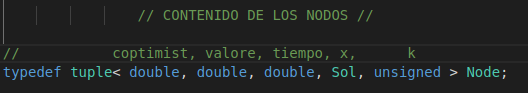
\includegraphics[scale=0.5]{contenido_nodo.png}
%     \caption{Contenido de los nodos}
%     \label{fig:nodo}
% \end{figure}

Entrando más en detalle con el funcionamiento de la función bt\_futoshiki(),
lo que se hace en el código es recorrer el tablero empezando por la superior 
izquierda y para cada posición se comprueban los números de 1 a N. Si el número es factible en esa posición, lo colocamos en la casilla con \verb|setCasilla()|
y llamaremos a la recursividad para seguir comprobando. Si no es factible, comprobamos el siguiente valor posible.

Tras llamar a la recursividad debemos ver si ha devuelto un resultado un resultado verdadero, en cuyo caso se ha encontradola solución y debemos
salir con \textit{true}.

Es importante tener en cuenta que si hemos  comprobado todos los valores posibles y no hay ninguno factible, estamos siguiendo una instanciación errónea y debemos devolver \textit{false}.

En el caso de que en la casilla ya haya un valor prefijado, debemos comprobar aún asi si es factible, pues si
no tendremos que volver hacia atrás. En ningún caso modificamos el valor de la casilla.

También es importante comentar el funcionamiento de \verb|factible()|. En esta función comprobamos si, al poner el valor en la casilla deseada:
 \begin{itemize}
    \item Si el número se repite en la casilla o en la columna.
    \item Si el número cumple las restricciones de \textit{"mayor que"} o \textit{"menor que"} con respecto a la 
        casilla anterior, pues al recorrer el tablero hacia abajo/derecha, comprobar con las casillas a nuestra derecha
        significa que estaríamos comprobando con casillas vacías, lo cual nos llevaría a resultados incorrectos.
 \end{itemize}

\subsubsection{Problemas durante la implementación}

Durante la implementación del algoritmo se dieron algunos problemas, que consiguieron ser solucionados para cumplir con la tarea. Los más destacable:

\begin{itemize}
    \item No se comprobaba si las llamadas recursivas devolvían la solución, con lo cual el algoritmo seguía aplicándose 
    una vez habiendo encontrado la solución.

    \item Al principio no se comprobaba si los números prefijados erán factibles, lo cual daba problemas en el momento 
    en que uno de estos tenía una una restricción binaria con una casilla adyacente. Esto llevaba a resultados incorrectos en 
    tableros como el de 6x6.

    \item No se devolvía falso cuando el algoritmo había descartado todos los números como soluciones factibles de una casilla, lo 
    cual llevaba a una indeterminación en la solución.
\end{itemize}

\subsection{Algoritmo AC3}

\subsubsection{Funciones y métodos}\label{ch:eisitris}

Para la implementación de este algoritmo, con el fin de seguir la estructura aprendida en clase, se implementaron 
nuevas clases al proyecto, además de añadir nuevos métodos y estructuras de datos.

Primero veamos las \textbf{clases} creadas:

\begin{itemize}
    \item \textbf{Clase nodo:} representa la estructura de datos de un nodo. Se compone de dos enteros que son
    sus coordenadas X e Y.
    \item \textbf{Clase arista:} representa la estructura de datos de una arista. Está compuesta de dos nodos A y B, y
    en el algoritmo consideraremos que la arista tiene dirección de A a B, aunque realmente la arista no tiene una dirección.
    
    \item \textbf{Clase matdominios:} representa el dominio de las casillas del tablero. Se compone de una matriz de 3 dimensiones, 
    donde la primera y segunda serán la fila y columna del tablero. La tercera dimensión representa los números que pueden estar en 
    esa posición. El valor en sí de la casilla [X][Y][Z] es \textit{"1"} o \textit{"0"} para indicar si el valor está o no en el dominio de esa casilla.
    En el código, se definirá como una \textbf{variable global}.
\end{itemize}

Ahora hablaremos de las \textbf{funciones} y \textbf{métodos} más importantes:

\begin{itemize}
    \item \verb|ejecutarAC3():| función base dada en la práctica, en ella se arregla el dominio
        del tablero siguiendo el esquema AC3.
    \item \verb|consistente():| en esta función se analiza la consistencia para un valor del nodo A
    con respecto a los valores del nodo B. Devolverá \textit{true} si hay algún valor del nodo que hace consistente al nodo A.
    
    \item \verb|enDominio():| método de la clase \textbf{matdominio} que analiza si un número se encuentra dentro del dominio
    de una casilla. Debemos especificar la fila, columna y valor a comprobar.

    \item \verb|sacarDominio:| método de la clase \textbf{matdominio} donde sacamos un valor dado del dominio de 
    la casilla (fila, columna) que le indiquemos.
    \item \verb|meterDominio:| método de la clase \textbf{matdominio} donde metemos un valor dado en el dominio de 
    la casilla (fila, columna) que le indiquemos.

    \item \verb|imprimirDominio():| método de la clase \textbf{matdominio} donde imprimimos por pantalla el dominio de la matriz de 
    dominios.
    
    \item También se utilizan los constructores, getters y setters de las clases.

\end{itemize}

En cuanto a \textbf{estructuras de datos} usadas, destacamos las siguientes:

\begin{itemize}
    \item \textbf{Nodo:} punto con coordenadas X e Y. 
    \item \textbf{Arista:} conexión entre dos nodos.
    
    \item \textbf{Matriz de dominios:} para saber que valores son accesibles para una casilla del tablero.
    \item \textbf{Colas de doble frente:} Las utilizaremos para guardar todas las aristas del tablero, y poder 
        ir haciendo el análisis en el algoritmo arista a arista. También utilizaremos otra para guardar aristas descartadas.
\end{itemize}

Entrando en detalle con el funcionamiento del algoritmo, lo primero que haremos será sacar del dominio todos los valores de casillas
prefijadas (dejándo también solo esos valores en el dominio de su casilla). Tras esto crearemos una matriz de nodos con todos los nodos
del tablero, y con ella iremos creando todas las aristas necesarias. Serán dos aristas (para cada direción) por cada par de nodos que 
estén en la misma fila o columna. Todas las aristas creadas se meten dentro de una cola.

Ahora, mientras la cola de descartes no quede vacía (haber analizado todas las aristas). Repetiremos el siguiente proceso:

\begin{itemize}
    \item Sacamos una arista del frente de la cola.
    \item De 1 a N comprobaremos si los valores están en el dominio del nodo A.
    \item Si esta en el dominio, comprobaremos si el valor es consistente con el nodo B, usando \verb|consistente()|.
    \item Si \textbf{no} es consistente, sacaremos el valor del dominio del nodo A, usando \verb|sacarDominio()|. 
    \item En caso de haber cambiado el dominio, debemos comprobar las aristas que se 
        han analizado previamente que apunten al nodo \textbf{A} actual. Esto lo haremos recurriendo 
        a una cola de descartes, donde se encuentran todas las aristas analizadas previamente.
    \item Si se queda vacío el dominio de un nodo, entonces no hay solución y salimos con false de la función.
\end{itemize}

Ahora comentaremos la función \verb|consistente()|, que es muy importante en cuanto a la resolución del algoritmo.

Esta función recibe un valor del nodo A y comprueba, para todos los valores del nodo B, las siguientes restricciones:

\begin{itemize}
\item Que no sean iguales.
\item En caso de que la distancia entre nodos sea 1, usamos la función \verb|getElement()|. 
    para ver la posición entre nodos y si hay una restricción. En este caso, comprobaremos si los valores cumplen esta restricción
    (de haberla).
\item Solo necesitamos que un valor cumpla con las restricciones para que la función devuelva \textit{true}.
\end{itemize}

Tras hacer los arreglos en el dominio con AC3, llamamos a  \verb|bt_futoshiki()|, que ha sido
 modificada para tener en cuenta la matriz de dominios (realizar comprobaciones sólo con números que 
 se encuentren dentro del dominio de una casilla) y esta resolverá el tablero, pero partiendo con un problema simplificado, lo que
 a priori debería mejorar el tiempo de resolución.



\subsubsection{Problemas durante la implementación}

Durante la implementación de AC3,  no hubo grandes problemas más allá de errores de compilación puntuales o 
problemas de \textit{segmentation fault}. Aunque si es cierto que hicieron falta muchas pruebas para llegar a la idea
de usar la cola de descartes o comprobar que las clases implementadas funcionaban bien con el código.

\subsection{Foward Checking}

\subsubsection{Funciones y métodos}

Para la implementación de Forward Checking, se reutilizaron varios métodos ya descritos en el apartado anterior \ref{ch:eisitris},
como por todos los métodos de la case \textbf{matdominio}. Las nuevas funciones y estructuras añadidas para este algoritmo son:

\begin{itemize}
    \item \textbf{Matriz de podados:} es una matriz del tipo \textbf{matdominios}, análoga a la matriz de dominio pero que se usa
        para saber, en cada nivel, que valores han sido eliminados del dominio. Se recurrirá a esta en caso de que queramos reestablecer 
        todos los valores eliminados en una determinada instanciación.
    \item \verb|ejecutarFC():| función dada para la práctica donde sacaremos los números prefijados de los dominios correspondientes y 
        donde rellenaremos el tablero una vez la función recursiva haya acabado.
    \item \verb|fc_futoshiki():| función recursiva y la principal del esquema de Forward Checking. 
    \item \verb|forward():| función que realiza el "razonamiento hacia adelante". 
    \item \verb|instanciar():| función que instancia un valor a una posición del dominio, sacando los demás posibles
        valores del dominio de esa casilla.
    \item \verb|restaurar():| en esta función usaremos la matriz de podados para volver a introducir todos los
        valores que fueron podados por la instanciación actual.
    \item \verb|consistente_fc():| es prácticamente la misma función que usamos para AC3, pero esta solo realiza la comparación
        entre un solo par de valores.     
\end{itemize}

Ahora, el funcionamiento del algortimo consiste en los siguientes pasos: 
\begin{itemize}
    
    \item Instanciamos uno de los valores posibles en la posición en la que nos encontramos.
    \item Razonamos hacia adelante, es decir, comprobamos si la instanciación que hemos propuesto es consistente
        con todas las demás casillas de la misma fila/columna. Si un valor no es consistente, lo eliminamos del dominio.
    \item Si no hay valores que consigan hacer cumplir el razonamiento hacia adelante, debemos restaurar todos los múmeros podados.
    \item Si el razonamiento no da problemas, llamamos a la recursividad para la siguiente casilla.
    \item En caso de que ningún valor de los probados de resultados, debemos restaurar todo lo podado a partir de la casilla actual y 
        volver hacia atrás.
    \item Si hemos llegado a la ultima posición, consideraremos que tenemos el resultado correcto.
    

\end{itemize}

\verb||
\textbf{}
\textit{}

\subsubsection{Problemas durante la implementación}

El principal problema que dio la implementación del algoritmo surge de no haber tenido en cuenta, al principio,
que se debían arreglar los dominios cuando realizamos la instanciación. Esto provocaba problemas a la hora de volver hacia atrás. Otro
problema fue considerar que el código solo restauraba si \verb|forward()| devolvía \textit{false}, cuando debía restaurar también si la 
llamada recursiva devolvía \textit{false}.

\begin{figure}[h]
    \centering
    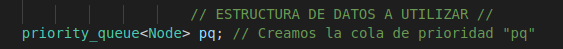
\includegraphics[scale=0.5]{cola_de_prior.png}
    \caption{Implementación de la cola de prioridad}
    \label{fig:colprior}
\end{figure}

\section{Estudio de los tiempos de ejecución}

En este apartado procederemos a comparar y comentar los distintos tiempos de ejecución y pasos entre las diferentes estrategias 
de resolución descritas durante la práctica. Además, a modo de experimentación, se han medido los tiempos resultantes de combinnar
las estrategias de AC3 y forward checking.

\begin{table}[H]
    \begin{center}
        \begin{tabular}{| c | c | c | c | c |}
            \hline
            \multicolumn{5}{ |c| }{Tiempos de ejecución (en \textbf{segundos})} \\ \hline
            Tablero & Backtracking & AC3 & Forward Checking & FC + AC3 \\ \hline
                        %BT             %AC      %FC     FCAC3
            4x4     &   0,000055    &    0,000472   &       &   \\
            5x5     &   0,005804    &    0,004638   &       &   \\
            6x6     &   0,000316    &    0,006238   &       &   \\
            7x7     &   0,118968    &    0,08557    &       &   \\ 
            9x9 (1) &               &    1,73674    &       &   \\
            9x9 (2) &    1,36732    &    0,173556   &       &   \\ \hline
        \end{tabular}
        \caption{Tiempos de ejecución para distintos tamaños de tablero}
        \label{tab:tiempo}
    \end{center}
\end{table} 

\begin{table}[H]
    \begin{center}
        \begin{tabular}{| c | c | c | c | c |}
            \hline
            \multicolumn{5}{ |c| }{Número de Pasos dados por casa algoritmo} \\ \hline
            Tablero & Backtracking & AC3 & Forward Checking & FC + AC3 \\ \hline
                        %BT         %AC      %FC     FCAC3
            4x4     &   33      &    26   &       &   \\
            5x5     &   7.362   &    26   &       &   \\
            6x6     &   181     &    37   &       &   \\
            7x7     &   232.989 &    183.504   &       &   \\ 
            9x9 (1) &           &    4.719.952   &       &   \\
            9x9 (2) & 3.005.483 &    357.409   &       &   \\ \hline
        \end{tabular}
        \caption{Pasos tomados para la solución distintos tamaños de tablero}
        \label{tab:pasos}
    \end{center}
\end{table} 

\end{document}